\documentclass[rascunho,xindy,sublist]{fei}
%\documentclass[rascunho,xindy,sublist]{report}

%\usepackage[utf8]{inputenc}
% \usepackage[table]{xcolor}

%\usepackage{biblatex}

%\usepackage[
%backend=biber,
%style=alphabetic,
%sorting=ynt
%]{biblatex}


\usepackage{pgfplots}
\pgfplotsset{compat=1.7}
\usepackage{pgfplots}
\usetikzlibrary{calc}
\usepackage{amsmath}
\usepackage{subcaption}
\usepackage[utf8]{inputenc}
\usepackage{comment}
\usepackage{acronym} 
\usepackage{glossaries}



% -- Configurações Iniciais

\author{Murilo Darce Borges Silva\\ Rodrigo Simões Ruy}

\title{Identificação de diferenças de desempenho entre sistemas robóticos reais, simulados e com software conteinerizado, utilizando Simulador Gazebo, ROS 2 e Docker.}
%\subtitulo{subtítulo}

%\cidade{Cidade}
%\instituicao{Instituição de Ensino}

%%%% -- Entradas Listas de Abreviaturas e Simbolos
%%%%%%%%%%%%%%%%%%%%%%%%%%%%%%%%%%%%%%%%%%%%%%%%%%%%%%%%%%%%%%%%%%%%%%%%%%%%%%%%%%%%%%%%%%%%%%%%%%%%%%%%%
%%%% -- Titulos - comentar caso a respectiva lista nao seja utilizada
\newglossaryentry{acro}{name={},description={\nopostdesc},sort=a} %Usado para alinhar a lista de abreviaturas
\newglossaryentry{geral}{name={Geral},description={\nopostdesc},sort=a}
\newglossaryentry{greek}{name={Letras gregas},description={\nopostdesc},sort=b}
\newglossaryentry{sub}{name={Subscritos},description={\nopostdesc},sort=c}

%% -- Abreviaturas
\newacronym[longplural=Computational Aided Design,parent=acro]{cad}{CAD}{Computational Aided Design}
\newacronym[longplural=Centro Universitário da FEI,parent=acro]{fei}{FEI}{Centro Universitário FEI}

%% -- Simbolos
%% -- Latin letters
%\newglossaryentry{}{parent=geral,type=symbols,name={},sort=a,description={}

\newglossaryentry{A}{parent=geral,type=symbols,name={\ensuremath{A}},sort=a,description={exchanger total heat transfer area, $m^2$}}
\newglossaryentry{G}{parent=geral,type=symbols,name={\ensuremath{G}},sort=g,description={exchanger flow-stream mass velocity, $kg/(s m^2)$}}
\newglossaryentry{f}{parent=geral,type=symbols,name={\ensuremath{j}},sort=j,description={friction factor, dimensionless}}

%% -- Greek letters
%\newglossaryentry{}{parent=geral,type=symbols,name={},sort=a,description={}
\newglossaryentry{deltap}{parent=greek,type=symbols,name={\ensuremath{\Delta P}},sort=p,description={pressure drop, $Pa$}}
\newglossaryentry{nu}{parent=greek,type=symbols,name={\ensuremath{\nu}},sort=b,description={specific volume, $m^3/kg$}}
\newglossaryentry{beta}{parent=greek,type=symbols,name={\ensuremath{\beta}},sort=b,description={ratio of free-flow area $A_{ff}$ and frontal area $A_{fr}$ of one side of exchanger, dimensionless}}

%% -- Subscripts
%\newglossaryentry{}{parent=geral,type=symbols,name={},sort=a,description={}
\newglossaryentry{fr}{parent=sub,type=symbols,name={\ensuremath{fr}},sort=fr,description={frontal}}
\newglossaryentry{in}{parent=sub,type=symbols,name={\ensuremath{i}},sort=in,description={inlet}}
\newglossaryentry{out}{parent=sub,type=symbols,name={\ensuremath{o}},sort=out,description={outlet}}
%%%%%%%%%%%%%%%%%%%%%%%%%%%%%%%%%%%%%%%%%%%%%%%%%%%%%%%%%%%%%%%%%%%%%%%%%%%

\makeindex
%\makeglossaries

\begin{document}

\maketitle
\begin{folhaderosto}

%Monografia apresentada ao Curso de Graduação em Ci\^{e}ncia da
%Computa\c{c}\~{a}o do Centro Universitário da FEI, como requisito
%parcial para a obten\c{c}\~{a}o do grau de Bacharel em Ci\^{e}ncia
%da Computa\c{c}\~{a}o.
Trabalho de Conclusão de Curso apresentado ao Centro Universitário FEI, como parte dos requisitos necessários para obtenção do título de Bacharel em Ciência da Computação. Orientado pelo Prof. Dr. Leonardo Anjoletto Ferreira.

\end{folhaderosto}

%\fichacatalografica

\orientador{Prof. Dr. Leonardo Anjoletto Ferreira}
\primeiroexaminador{Prof. Dr. Plinio Thomaz Aquino Junior}
\segundoexaminador{Prof. Dr. Fagner de Assis Moura Pimentel}
\dataaprovacao{06/06/2025}

\begin{folhadeaprovacao}

Trabalho de Conclusão de Curso apresentado ao Centro Universitário FEI, como parte dos requisitos necessários para obtenção do título de Bacharel em Ciência da Computação.

\end{folhadeaprovacao}

%\dedicatoria{A quem eu quero dedicar o texto.}
%\begin{agradecimentos}
%\end{agradecimentos}
%\epigrafe{Science never solves a problem without creating ten more}{George Bernard Shaw \nocite{george_bernard}}

\centerline{\bfseries RESUMO}
\label{resumo}
\vspace{8mm}

Conteinerização é uma ferramenta muito útil quando se lida com projetos que precisam de diferentes dependências ou programas que podem ter conflitos entre si, que precisam de uma grande quantidade de configuração inicial, ou que precisam de portabilidade. Isso a torna perfeita para projetos de robótica, mas os impactos do seu uso e suas peculiaridades em situações reais ainda não estão documentadas, o que é justamente oque este projeto propõe fazer. Haverão 2 partes para este projeto, a primeira parte será uma avaliação do desempenho em uma simulação utilizando Gazebo, e a segunda parte será a avaliação do desempenho de um turtlebot real.  

Palavras-chave: Robótica, ROS, Docker, Conteinerização

\centerline{\bfseries ABSTRACT}
\label{abstract}
\vspace{8mm}

Containerization is a very useful tool when dealing with projects that require different dependencies or programs that may conflict with each other, require a lot of initial configuring, or demand portability. This made it perfect for robotics projects, but the impacts of its usage and quirks in real scenarios are still undocumented, which is what this project aims to do. The project will have 2 parts, the first will be an assessment of the performance of a simulation using Gazebo, and the second part will be an assessment of the performance of a real turtlebot.

Keywords: Robotics, ROS, Docker, Containerization

% este comando é para ser descomentado apenas na versao final
%\listoffigures

% este comando é para ser descomentado apenas na versao final
%\listoftables

% este comando é para ser descomentado apenas na versao final
%\listofalgorithms

% este comando é para ser descomentado apenas na versao final
%\glsaddall

% este comando é para ser descomentado apenas na versao final
%\printglossaries

\tableofcontents

% este arquivo aqui pode ser descomentado quando forem fazer a introdução
 \chapter{INTRODUÇÃO}
\label{intro}

\begin{comment}
\emph{Questão a ser respondida pela Introdução: O que você fez? E por que você fez isso?}
Na introdução devemos ajudar o leitor a entender o motivo / importância da pesquisa e o que ela está contribuindo para a área. Portanto, indique a motivação (ou motivações) para fazer a pesquisa e o que ela contribuirá para o campo.

Dê também ao leitor uma breve descrição sobre a área de pesquisa de forma geral e ampla e, então, reduza ao foco específico do trabalho, oferecendo informações detalhadas sobre o tópico pesquisado.

Deixe claro quais são os objetivos da pesquisa. 

Pode-se, no final da introdução, apresentar ainda a estrutura do trabalho, indicando como ele está organizado e os tópicos que serão abordados em cada seção subsequente.

Nos últimos anos, a globalização e as transformações tecnológicas vêm redefinindo a estrutura do mercado de trabalho em todo o mundo [1]. Essas mudanças têm afetado profundamente a segurança do emprego e as condições de trabalho dos indivíduos. O objetivo deste trabalho é investigar o impacto da automação e da inteligência artificial na precarização do trabalho, analisando como essas tecnologias têm contribuído para o aumento da informalidade e da desigualdade no mercado de trabalho. Este estudo é relevante em um contexto em que a preocupação com a segurança no emprego e a equidade está no centro das discussões globais.

Nos últimos anos, a Inteligência Artificial (IA) se consolidou como uma das tecnologias mais promissoras e transformadores do nosso tempo [1]. A capacidade das máquinas de aprender e tomar decisões de forma
autônoma tem aplicações em uma variedade de setores, desde a medicina até o transporte [2]. Este estudo tem como objetivo investigar o uso da IA na otimização de sistemas de recomendação em plataformas de streaming de vídeos. Com o crescente volume de conteúdo disponível, tornou-se crucial para as empresas de streaming entender as preferências dos usuários e oferecer recomendações personalizadas. Esta pesquisa é relevante não apenas do ponto de vista da indústria de entretenimento,
mas também do ponto de vista da pesquisa em IA, pois aborda desafios técnicos significativos.
\end{comment}



A conteinerização é uma ferramenta poderosa no campo de desenvolvimento e implementação, disponibilizando certa camada de isolamento entre componentes de um projeto, assegurando que estes não irão conflitar, seja por funções internas ou dependências de versões diferentes sendo utilizadas. No campo da robótica, conteinerização é vista como uma técnica para facilitar o desenvolvimento, portabilidade e consistência em projetos de robótica, mas não foram feitas pesquisas detalhando a integração destes projetos com Docker e seus efeitos no desempenho de um robô físico. A proposta do projeto é justamente esta: integrar ROS 2 e Docker, explicando os passos utilizados e comparando o desempenho com e sem conteinerização, sendo dividido em 2 partes: em um simulador Gazebo, e em um robô Turtlebot real.
\begin{comment}
    \begin{itemize}
    \item Contexto
    \begin{enumerate}
        \item Como esse tópico se encaixa no contexto da área de pesquisa?\\
        R: Se encaixa na pesquisa pois estamos utilizando técnicas da área da ciência da computação para implementar e avaliar o desempenho de ROS + Docker.
        \item Qual a relevância do tópico escolhido para a área de estudo?\\
        R: O trabalho é relevante pois pode ajudar futuros projetos utilizando ROS+Docker, ao evidenciar certas falhas e/ou perdas de desempenho relacionado com essa integração
        \item Quais eventos históricos e/ou recentes que contextualizam esse tópico?\\
        R: O crescimento do uso de containers em projetos com grande quantidade de complexidade/dependências [colocar artigo aqui]
    \end{enumerate}
    \item Problema de pesquisa
    \begin{enumerate}
        \item Qual a questão central que seu TCC se propõe a abordar?\\
        R: Diferenças de desempenho relacionada à integração Docker, além de possível incompatibilidades/peculiariades relacionadas.
        \item Por que esse problema é significativo ou merece investigação?\\
        R: Pois sem saber destas diferenças, é difícil fazer a decisão de qual partes do projeto podem ser integradas a Docker, e qual os possíveis riscos.
        \item Existem lacunas na literatura existente relacionada a esse problema?\\
        R: Sim, já foram feitos vários estudos relacionados ao desempenho do ROS+Docker em simulações, ou sua inicialização [colocar artigo aqui], mas não no robô físico.
    \end{enumerate}
    \item Objetivos
    \begin{enumerate}
        \item Quais são os principais objetivos do seu TCC?\\
        R: Encontrar e avaliar diferenças na performance e compatibilidade de projetos ROS e ROS+Docker
        \item Como seus objetivos estão relacionados ao problema de pesquisa?\\
        R: Ter estes dados irá facilitar a avaliação e desenvolvimento de futuros projetos ROS+Docker.
        \item O que você espera alcançar com esta pesquisa?\\
        R: A obtenção de dados relevantes à decisão de integrar Docker ao projeto, e quais partes deste podem ganhar com esta integração.
    \end{enumerate}
    \item Justificativa
    \begin{enumerate}
        \item Por que é importante abordar esse problema de pesquisa?\\
        R: 
        \item Quais são as implicações práticas e teóricas da sua pesquisa?\\
        R: 
        \item Como sua pesquisa contribuirá para o conhecimento existente na área?\\
        R: 
    \end{enumerate}
    \item Hipótese
    \begin{enumerate}
        \item Qual é a suposição sendo feita com base na revisão da literatura?\\
        R: Que existem diferenças que não se mostram em simulações.
        \item Como sua suposição se relaciona ao problema de pesquisa?\\
        R: 
        \item Como você pretende testar ou validar essa hipótese?\\
        R: Utilizando métricas como tempo e aproveitamento para medir o desempenho, e uma medição binária para compatibilidades
    \end{enumerate}
\end{itemize}
\end{comment}


\section{OBJETIVO}
Documentar e avaliar o desempenho do robô simulado e do robô real quando comparados à sua implementação com e sem conteinerização.

\begin{comment}
\section{ESTRUTURA DO TRABALHO}

O restante deste trabalho é dividido da seguinte maneira: na Seção 2, serão
apresentados todos os conceitos utilizados e relacionados ao tema abordado, para que o leitor possa entender com clareza as técnicas que estão sendo tratadas no trabalho e compreender os termos que serão descritos posteriormente.

Na Seção 3, os trabalhos relacionados disponíveis na literatura, com o objetivo de apresentar o cenário atual de pesquisa da área.
 
A Seção 4 detalhará a metodologia que será utilizada para o desenvolvimento deste trabalho, demonstrando as técnicas que serão utilizadas e os passos a serem realizados para atingir o objetivo final.

O Seção 5 irá expor o que os autores deste trabalho esperam ao longo do desenvolvimento e após a implementação da metodologia proposta.

\end{comment}



% este arquivo aqui pode ser descomentado quando forem fazer os conceitos
\chapter{CONCEITOS FUNDAMENTAIS} \label{conceitos}

\begin{comment}
\emph{Questão a ser respondida pelos Conceitos: Quais são os fundamentos teóricos relevantes?}
Aqui define-se os principais termos e conceitos que serão utilizados ao longo do trabalho. Para essa seção é recomendada a utilização de livros e artigos já consolidados na literatura. Todos os parágrafos dessa seção devem ter pelo menos uma citação. 
\end{comment}

Para o entendimento de alguns softwares e o porquê de estarem sendo utilizados, existem alguns conceitos que devem ser compreendidos para o total entendimento do projeto. Estes conceitos são:

\textbf{Conteinerização:} Uma forma de virtualização feita para ser mais rápida e flexível que a emulação, é um processo de implantação que consegue ser executado em diversos dispositivos e sistemas operacionais, isso ocorre pelo fato de que um contêiner consegue armazenar os arquivos e bibliotecas para ser executado, permitindo um usuário executar uma aplicação de outro sistema operacional no sistema operacional que o mesmo possua, além disso, o contêiner permite que falhas ocorram sem afetar outros processos que não estão agrupados no mesmo. \cite{Wen2023}

\begin{comment}
    \textbf{Conteinerização:} Uma forma de virtualização feita para ser mais rápida e flexível que emulação, mas ainda ter sua consistência e isolamento do Sistema Operacional principal \cite{Wen2023}.

    A conteinerização é um processo de implantação de software que agrupa o código de uma aplicação com todos os arquivos e bibliotecas de que ela precisa para ser executado em qualquer infraestrutura. Tradicionalmente, para executar qualquer aplicação em seu computador, era necessário instalar a versão que correspondia ao sistema operacional da sua máquina. Por exemplo, você precisava instalar a versão Windows de um pacote de software em uma máquina Windows. No entanto, com a conteinerização, você pode criar um único pacote de software, ou contêiner, que é executado em todos os tipos de dispositivos e sistemas operacionais. 
\end{comment}

\textbf{Meta-sistema operacional:} Um meta-sistema operacional se trata de um sistema operacional para robôs, o mesmo realiza todas as funções que um sistema operacional faz. O mesmo possui bibliotecas e ferramentas que executam códigos em multiplos computadores. Este sistema operacional é utilizado em robôs...
%https://wiki.ros.org/ROS/Introduction

\begin{comment}
    \textbf{Meta-sistema operacional:} É um sistema operacional que é desenvolvido e executado em outro sistema operacional, permitindo que diferentes processos possam se comunicar durante a execução. Este conceito é aplicado para o ROS.

     It also provides tools and libraries for obtaining, building, writing, and running code across multiple computers. ROS is similar in some respects to 'robot frameworks,' such as Player, YARP, Orocos, CARMEN, Orca, MOOS, and Microsoft Robotics Studio.
\end{comment}
%https://stackoverflow.com/questions/15150599/what-is-the-difference-between-operating-system-and-meta-operating-system#:~:text=The%20basic%20difference%20is%20that,with%20each%20other%20at%20runtime.

\textbf{Middleware:} Uma camada de software que conecta as aplicações a um sistema operacional, permitindo uma comunicação e compartilhamento de dados mais simples entre os componentes de um sistema, esta facilidade permite que os desenvolvedores foquem no desenvolvimento das principais funções de uma aplicação, pois a comunicação entre a aplicação e o sistema operacional está sendo feita pelo middleware.
%Middleware é uma camada de software que conecta o sistema operacional a aplicações, dados e usuários. Ele disponibiliza serviços e recursos compartilhados, como single sign-on (SSO) e gerenciamento de interfaces de programação de aplicações (APIs). Os desenvolvedores podem contar com o middleware para fornecer integrações consistentes e simplificadas entre os componentes da aplicação. Assim, os profissionais podem se concentrar na criação de funcionalidades essenciais, no tempo em que estariam conectando essas funções a diferentes endpoints e ambientes, como sistemas legados.

\textbf{DDS:} Um protocolo middleware e uma API para conexão centrada em dados, este protocolo integra os componentes de um sistema que muitas aplicações precisam, como arquitetura escalar, confiabilidade e prover conectividade de dados de baixa latência. Este protocolo foi criado pela OMG.
%https://www.dds-foundation.org/what-is-dds-3/
%The OMG Data Distribution Service (DDS™) is a middleware protocol and API standard for data-centric connectivity from the Object Management Group® (OMG®). It integrates the components of a system together, providing low-latency data connectivity, extreme reliability, and a scalable architecture that business and mission-critical Internet of Things (IoT) applications need.

%In a distributed system, middleware is the software layer that lies between the operating system and applications. It enables the various components of a system to more easily communicate and share data. It simplifies the development of distributed systems by letting software developers focus on the specific purpose of their applications rather than the mechanics of passing information between applications and systems.

\subsection{FERRAMENTAS}
Para o desenvolvimento do projeto, serão utilizados softwares e ferramentas para que os testes possam ser realizados e analisados. As ferramentas utilizadas serão:

\textbf{Docker:} É uma plataforma utilizada para desenvolvimento, envio e funcionamento de aplicações de maneira separada da infraestrutura por conta da conteinerização, por conta deste fator o usuário consegue gerir as aplicações da mesma maneira que gera sua infraestrutura, outro fator importante é que o Docker permite que as aplicações desenvolvidas sejam testadas e executadas com menos atraso do que a maneira convencional. Contêineres são bons para fluxos de integrações e entregas de trabalho contínuas.\cite{dck2025}
 %Docker is an open platform for developing, shipping, and running applications. Docker enables you to separate your applications from your infrastructure so you can deliver software quickly. With Docker, you can manage your infrastructure in the same ways you manage your applications. By taking advantage of Docker's methodologies for shipping, testing, and deploying code, you can significantly reduce the delay between writing code and running it in production.
%(Fast, consistent delivery of your applications) Docker streamlines the development lifecycle by allowing developers to work in standardized environments using local containers which provide your applications and services. Containers are great for continuous integration and continuous delivery (CI/CD) workflows.
%\newpage

\textbf{ROS2(Robot Operating System 2):} É um meta-sistema operacional de código aberto utilizado para auxiliar a desenvolver aplicações para robôs, o mesmo possui serviços que outros sistemas operacionais normalmente possuem, mas com o foco maior para a área da robótica, facilitando comunicação entre processos, funções que se comunicam com as demais e entre muitos outros. Para o desenvolvimento do projeto, será utilizado o ROS 2 que mantém o conceito modular e distribuido, mas possui melhorias e mais funcionalidades que o ROS original (Observar figura \ref{fig:ROS25}) \cite{ros2025}

%The Robot Operating System (ROS) is a set of software libraries and tools that help you build robot applications. From drivers to state-of-the-art algorithms, and with powerful developer tools, ROS has what you need for your next robotics project. And it's all open source.

%https://wiki.ros.org/ROS/Introduction
%ROS is an open-source, meta-operating system for your robot. It provides the services you would expect from an operating system, including hardware abstraction, low-level device control, implementation of commonly-used functionality, message-passing between processes, and package management. It also provides tools and libraries for obtaining, building, writing, and running code across multiple computers. ROS is similar in some respects to 'robot frameworks,' such as Player, YARP, Orocos, CARMEN, Orca, MOOS, and Microsoft Robotics Studio.
\textbf{Gazebo Simulator:} É um software usado para desenvolver simulações, possui diversos projetos de código aberto para que os interessados possam utilizar e desenvolver suas próprias simulações. Neste software estão presentes também diversos modelos, tanto como objetos como também robôs.(Observar figura \ref{fig:gzb25}) \cite{gzb2025}


% https://gazebosim.org/home Gazebo é uma coleção de bibliotecas de software de código aberto projetadas para simplificar o desenvolvimento de aplicações de alto desempenho. O público-alvo do Gazebo são desenvolvedores, designers e educadores de robôs. No entanto, o Gazebo foi estruturado para atender a diversos casos de uso. Cada biblioteca dentro do Gazebo possui dependências mínimas, permitindo que sejam usadas em tarefas que vão desde a resolução de transformações matemáticas até a codificação de vídeo, simulação e gerenciamento de processos. Basta escolher as bibliotecas necessárias para sua aplicação sem se comprometer com um ecossistema inteiro.
\textbf{TurtleBot3 Burger:} É um robô customizável de preço acessível ao público baseado no modelo ROS para ser utilizado como um material educativo, de pesquisas, entretenimento pessoal e etc, é um robô que foi desenvolvido com o intuito de ser barato, por conta disto, o mesmo não possui uma grande funcionalidade ou qualidade, mas o mesmo compensa na relação da quantidade de aplicações que o mesmo consegue realizar.(Observar figura \ref{fig:tbt3b25}) \cite{turtlebot3_manual}

\textbf{Fast DDS:} Implementação de DDS feita em c++, possui uma biblioteca que oferece uma API e protocolo de comunicação que disponibiliza um modelo Publisher-Subscriber centrado em dados (DCPS). Este modelo visa ser eficiente e confiável para distribuir as informações para o sistema em tempo real.
%https://fast-dds.docs.eprosima.com/en/stable/02-formalia/titlepage.html#
%eProsima Fast DDS is a C++ implementation of the DDS (Data Distribution Service) Specification, a protocol defined by the Object Management Group (OMG). The eProsima Fast DDS library provides both an Application Programming Interface (API) and a communication protocol that deploy a Data-Centric Publisher-Subscriber (DCPS) model, with the purpose of establishing efficient and reliable information distribution among Real-Time Systems.


\textbf{Cyclone DDS:} Implementação de DDS com alto desempenho, permite que os desenvolvedores que o utilizam possam criar "gêmeos" digitais das entidades de seus sistemas permitindo compartilhar estados, eventos, fluxos de dados e mensagens pela rede em tempo real, visa ser rápido, consistente e seguro.
%https://cyclonedds.io/
%Building Portable & Interoperable Distributed Datacentric Systems Cyclone DDS is a high performing, OMG-DDS standard based data sharing technology which allows system designers to create digital twins of their systems' entities to share their states, events, data-streams and messages on the network in real-time and fault-tolerant way.

%TurtleBot is a low-cost, personal robot kit with open-source software. TurtleBot was created at Willow Garage by Melonee Wise and Tully Foote in November 2010. With TurtleBot, you’ll be able to build a robot that can drive around your house, see in 3D, and have enough horsepower to create exciting applications.
%The TurtleBot kit consists of a mobile base, 2D/3D distance sensor, laptop computer or SBC(Single Board Computer), and the TurtleBot mounting hardware kit. In addition to the TurtleBot kit, users can download the TurtleBot SDK from the ROS wiki. TurtleBot is designed to be easy to buy, build, and assemble, using off the shelf consumer products and parts that easily can be created from standard materials. As an entry level mobile robotics platform, TurtleBot has many of the same capabilities of the company’s larger robotics platforms, like PR2.
%TurtleBot3 is made up of modular plates that users can customize the shape. Available in three types: small size Burger and medium size Waffle, Waffle Pi. TurtleBot3 consists of a base, two Dynamixel motors, a 1,800mAh battery pack, a 360 degree LIDAR, a camera(+ RealSense camera for Waffle kit, + Raspberry Pi Camera for Waffle Pi kit), an SBC(single board computer: Raspberry PI 3 and Intel Joule 570x) and a hardware mounting kit attaching everything together and adding future sensors. Turtlebot3 was released on May 2017.



%The TurtleBot3 in specific is a small, affordable, and customizable, ROS-based mobile robot for use in education, research, hobby projects, and product prototyping. The goal of TurtleBot3 is to provide a low cost, highly flexible robotics development platform without having to sacrifice functionality and quality, while at the same time offering enough expandability to fit a wide variety of complex robotics applications. The TurtleBot3 can be customized in various ways using simple mechanical components and through the use of upgraded electronic components including custom computers and sensors. In addition, the TurtleBot3 has continued to evolve it’s out of the box performance by continually upgrading the included cost-effective and small-sized SBC suitable for robust embedded systems. The TurtleBot3’s core technology of SLAM, Navigation and Manipulation makes it suitable for a wide variety of research and service robotics applications.
\begin{figure}[htb]
    \centering
    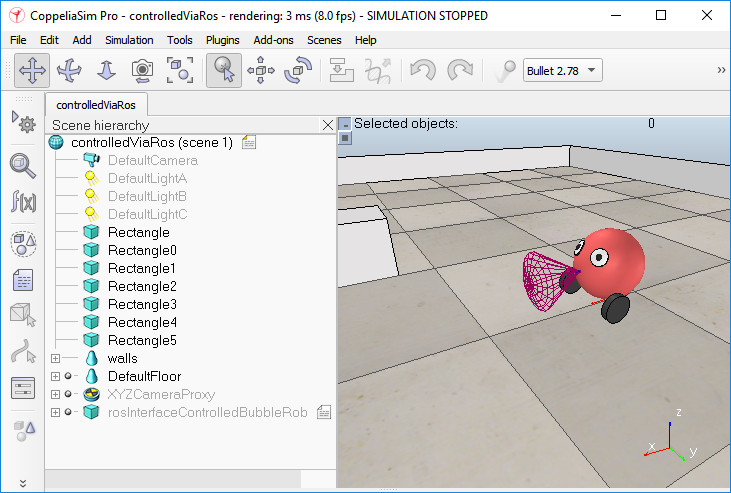
\includegraphics[width=0.5\linewidth]{Figures/ROS.png}
    \caption{TROCAR ESSA IMAGEM \cite{cop2020}}
    \label{fig:ROS25}
\end{figure}

\newpage
\begin{figure}[htb]
    \centering
    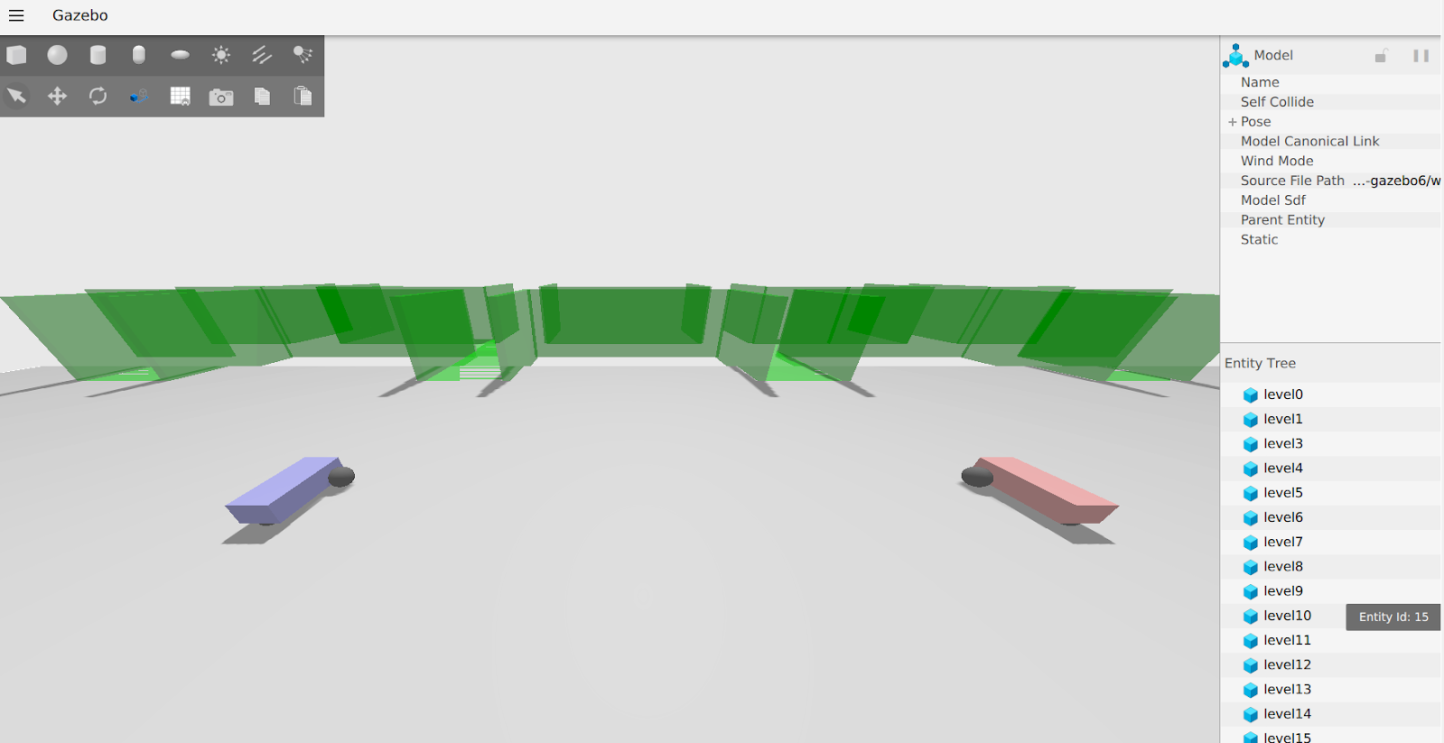
\includegraphics[width=0.5\linewidth]{Figures/gazebo.png}
    \caption{Exemplo utilizando o Gazebo Simulator \cite{gzb2025}}
    \label{fig:gzb25}
\end{figure}

\begin{figure}[htb]
    \centering
    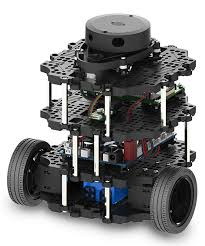
\includegraphics[width=0.3\linewidth]{Figures/TurtleBot3.jpg}
    \caption{TurtleBot3 Burger \cite{tbt2025}}
    \label{fig:tbt3b25}
\end{figure}

% este arquivo aqui pode ser descomentado quando forem fazer os trabalhos relacionados
\chapter{TRABALHOS RELACIONADOS} \label{trabs}
\begin{comment}
\emph{Questão a ser respondida pelos Trabalhos relacionados: O que os outros já fizeram?}
Seção em que serão descritos os trabalhos do estado da arte sobre o tema escolhido. Essa seção deve ser feita com base nos artigos mais novos e mais relevantes da área, seguindo o procedimento detalhado em Revisão Bibliográfica. Nessa seção todos os parágrafos devem também ter citação.

Exemplos de citação: 

Citação online (\verb!\citeonline{citacao_do_arquivo_bib}!): segundo \citeonline{dperico2021}, dado um grupo de agentes autônomos egocêntricos que percebem o ambiente por meio de câmeras independentes, o desenvolvimento de algoritmos capazes de produzir um conjunto de comandos de alto nível (envolvendo direções qualitativas: por exemplo, mover para a esquerda, seguir em frente) capaz de guiar um robô privado de sentido para um local de destino é possível. Citação tradicional (\verb!\cite{citacao_do_arquivo_bib}!): \cite{dperico2021}.

Mais detalhes sobre a seção Trabalhos Relacionados:
\url{https://encurtador.com.br/ozNY9}
\end{comment}
Para o desenvolvimento do projeto, foram relacionados alguns artigos que auxiliam no desenvolvimento do mesmo, O artigo "Bare-Metal vs. Hypervisors and Containers: Performance Evaluation of Virtualization Technologies for Software-Defined Vehicles"\cite{Wen2023} auxilia com relação ao entendimento da conteinerização em sistemas embarcados e também com relação ao seu desempenho. No artigo, é detalhada a utilização de diferentes formas de conteinerização e seu efeito no desempenho em diferentes tipos de hardware.

O artigo "Docker Performance Evaluation across Operating Systems"\cite{SMKD2024} auxilia no entendimento dos conceitos de avaliação do Docker com relação a outros sistemas operacionais, para verificar a diferença entre os sistemas operacionais o mesmo utilizou os recém instalados Sistemas Operacionais que eram MacOS ventura, Ubuntu 22.04 e Windows 10 rodando em um MacBook Pro 13, os testes consistiam em "estressar" o Docker com relação à CPU, Rede e na resiliência do mesmo, este artigo auxilia no entendimento com relação aos tipos de testes que podem ser realizados para analisar o desempenho dos robôs nas simulações e nos testes físicos.

Para a parte física, o artigo "Design and Ground Performance Evaluation of a Multi-Joint Wheel-Track Composite Mobile Robot for Enhanced Terrain Adaptability"\cite{Gao2023} tem o intuito de propor um robô multi-junta que consiga circular em vários tipos de terrenos, o artigo se diferencia por ser um robô com pernas, mas demonstra maneiras de se analisar o desempenho do robô auxiliando com relação à análise e entendimento de desempenho de um robô físico e sobre as suas causas.

%The tracked-wheeled mobile robot has gained significant attention in military, agricultural, construction, and other fields due to its exceptional mobility and off-road capabilities. Therefore, it is an ideal choice for reconnaissance and exploration tasks. In this study, we proposed a multi-jointed tracked-wheeled compound mobile robot that can overcome various terrains and obstacles. Based on the characteristics of multi-jointed robots, we designed two locomotion modes for the robot to climb stairs and established the kinematics/dynamics equations for its land movement. We evaluated the robot’s stability during slope climbing, its static stability during stair climbing, and its ability to cross trenches. Based on our evaluation results, we determined the key conditions for the robot to overcome obstacles, the maximum height it can climb stairs, and the maximum width it can cross trenches. Additionally, we developed a simulation model to verify the robot’s performance in different terrains and the reliability of its stair-climbing gait. The simulation results demonstrate that our multi-jointed tracked-wheeled compound mobile robot exhibits excellent reliability and adaptability in complex terrain, indicating broad application prospects in various fields and space missions.



% este arquivo aqui pode ser descomentado quando forem fazer a metodologia
\chapter{METODOLOGIA}

A metodologia (Observada na \ref{fig:Fluxograma}) é dividida em 2 partes. Na primeira parte, será utilizada uma simulação no gazebo simulator. A simulação possuirá um ambiente para testar o desempenho de um robô turtlebot. Ocorrerão dois testes, no primeiro teste o robô utilizará apenas ROS 2 enquanto no segundo teste o robô utilizará ROS 2 e Docker. Após a análise[EXPLICAR COMO É FEITA A ANÁLISE] do desempenho nos testes, os dados serão armazenados, analisados e finalmente comparados.
Na segunda parte, ao invés de uma simulação, será utilizado um robô turtlebot real. Os testes são semelhantes aos aplicados na primeira parte, onde o primeiro teste será realizado apenas com ROS 2 enquanto o segundo será realizado com ROS 2 e Docker juntos, para que assim os dados de desempenho possam ser coletados, analisados e então comparados.
As arenas que serão utilizadas na simulação serão baseadas em possíveis arenas que serão montadas na FEI na sala k404. A mesma possui uma arena que pode ser montada e um robô TurtleBot 3 Burger para a realização dos testes, assim será desenvolvida uma simulação com uma arena baseada na arena existente na instituição. A arena possui um caminho, mas o mesmo pode [COLOCAR UMA IMAGEM DA ARENA DA K404] ser alterado com algumas placas que funcionam como paredes, essas paredes permitem a criação de um caminho diferente para o robô podendo ser feito um labirinto, assim seria desenvolvida uma simulação com a mesma ideia para que se pudesse obter dados com uma relação maior. Com relação à parte física, seriam utilizados tanto o robô quanto a arena física para que pudessem ser executados os testes necessários para se adquirir os dados para então analisá-los e compararmos.

\begin{figure}[htb]
    \centering
    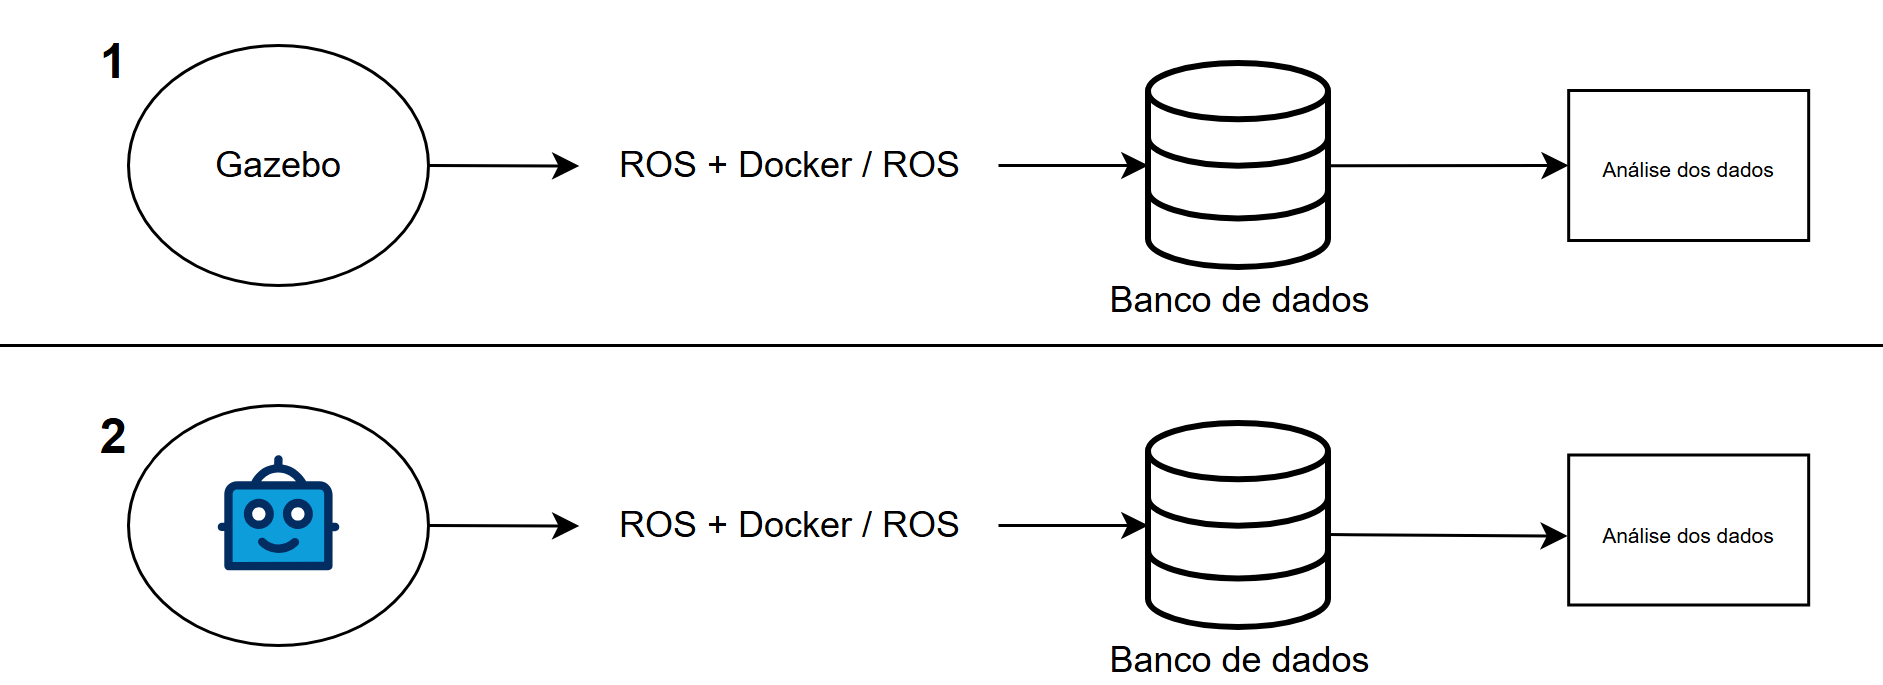
\includegraphics[width=0.9\linewidth]{Figures/FluxogramaTCC.png}
    \caption{Fluxograma do projeto[NECESSITA SER REFERENCIADO]}
    \label{fig:Fluxograma}
\end{figure}

% este arquivo aqui pode ser descomentado quando forem fazer a proposta experimental
\chapter{EXPERIMENTOS E RESULTADOS[EXPLICAR FIGURAS]}
\label{experimentos}
\begin{comment}
    

\emph{Questão a ser respondida pelos Experimentos e Resultados: O que foi encontrado?}
A seção de experimentos e resultados organiza e simplifica as descobertas da pesquisa para os leitores.

Concentre-se nos detalhes que são mais relevantes para avaliar o que foi estudado.
Faça comparações e descreva tendências quando apropriado (por exemplo, esse método teve acurácia melhor que aquele outro).
Utilize gráficos, tabelas, figuras para ajudar na apresentação dos resultados.
Evite qualquer interpretação ou explicação para os resultados.

Nesse capítulo é interessante ter uma seção falando sobre limitações que foram encontradas durante o projeto. Entretanto, a ideia não é justificar o que não deu tempo de fazer, mas sim elencar possíveis trabalhos futuros que essas limitações derivam.

É muito relevante colocar artigos e ou congressos que o projeto foi publicado e apresentado.
\end{comment}
Foram feitos testes para implementar a parte simulada proposta, sendo utilizado o manual \cite{turtlebot3_manual} e pacotes \cite{turtlebot3_github} disponíveis pelo grupo ROBOTIS, tornando o desenvolvimento desta parte rápido. A utilização e desenvolvimento dos projetos ROS2 dentro do Docker foi facilitada pela utilização de workflows no GitHub, onde as imagens de teste foram automaticamente construídas e publicadas como pacotes no repositório, o que reduziu o tempo do processo de construir as imagens localmente, que demorava de 20+ minutos para no máximo 5 minutos, além de também as disponibilizar para outros usarem.

%O erro é o \cite do github
%Foram feitos testes \cite{github_tcc_docker} para implementar a parte simulada proposta, sendo utilizado o manual \cite{turtlebot3_manual} e pacotes \cite{turtlebot3_github} disponíveis pelo grupo ROBOTIS, tornando o desenvolvimento desta parte rápido. A utilização e desenvolvimento dos projetos ROS2 dentro do Docker foi facilitada pela utilização de workflows no GitHub, onde as imagens de teste foram automaticamente construídas e publicadas como pacotes no repositório, o que reduziu o tempo do processo de construir as imagens localmente, que demorava de 20+ minutos para no máximo 5 minutos, além de também as disponibilizar para outros usarem.

Houve certas dificuldades para integrar o ROS2 dentro do contêiner Docker com o ROS2 nativo, que lidaria com a simulação Gazebo. Foi descoberto que o middleware utilizado por padrão pelo ROS2 Humble, FastDDS, não interage de forma consistente com Docker. Ele era capaz de compartilhar os tópicos entre os ambientes, mas causava falha na publicação e recebimento de mensagens, não mostrando nenhuma.

Para solucionar isso, o FastDDS foi substituído por outro middleware disponível para ROS2 Humble, CycloneDDS, o qual foi utilizado especificamente no contêiner Docker.

\begin{figure}[htb]
    \centering
    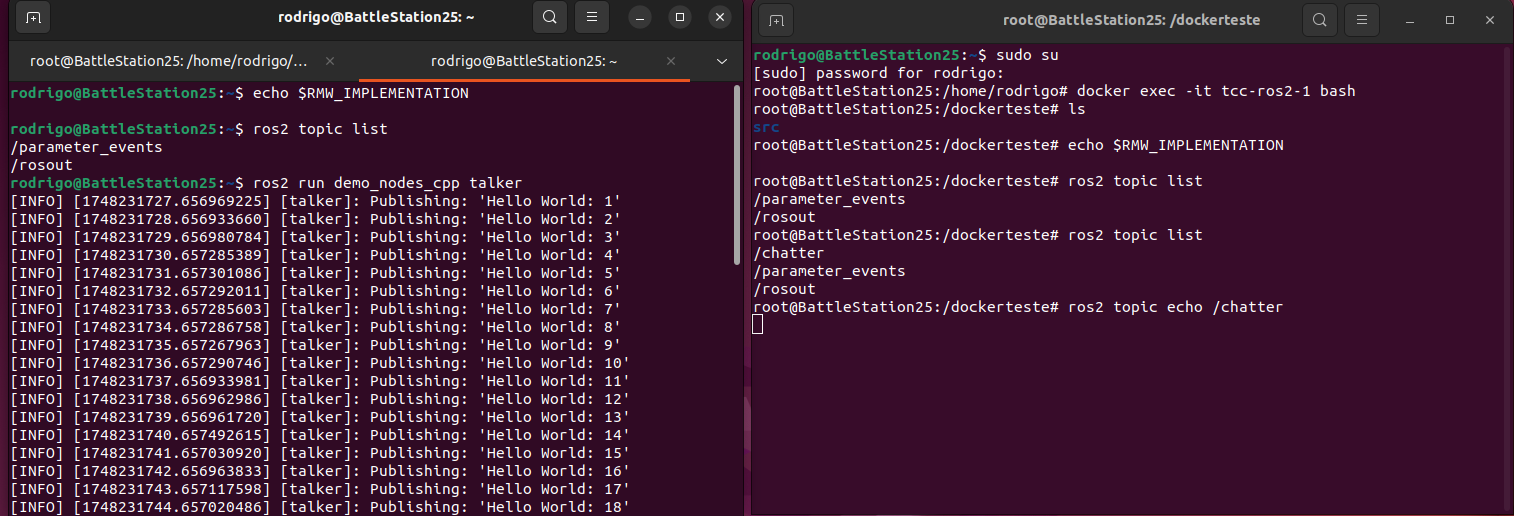
\includegraphics[width=1\linewidth]{Figures/TestePadraoFalha.png}
    \caption{Falha utilizando RMW padrão (FastDDS)}
    \label{fig:enter-label}
\end{figure}
\begin{figure}[htb]
    \centering
    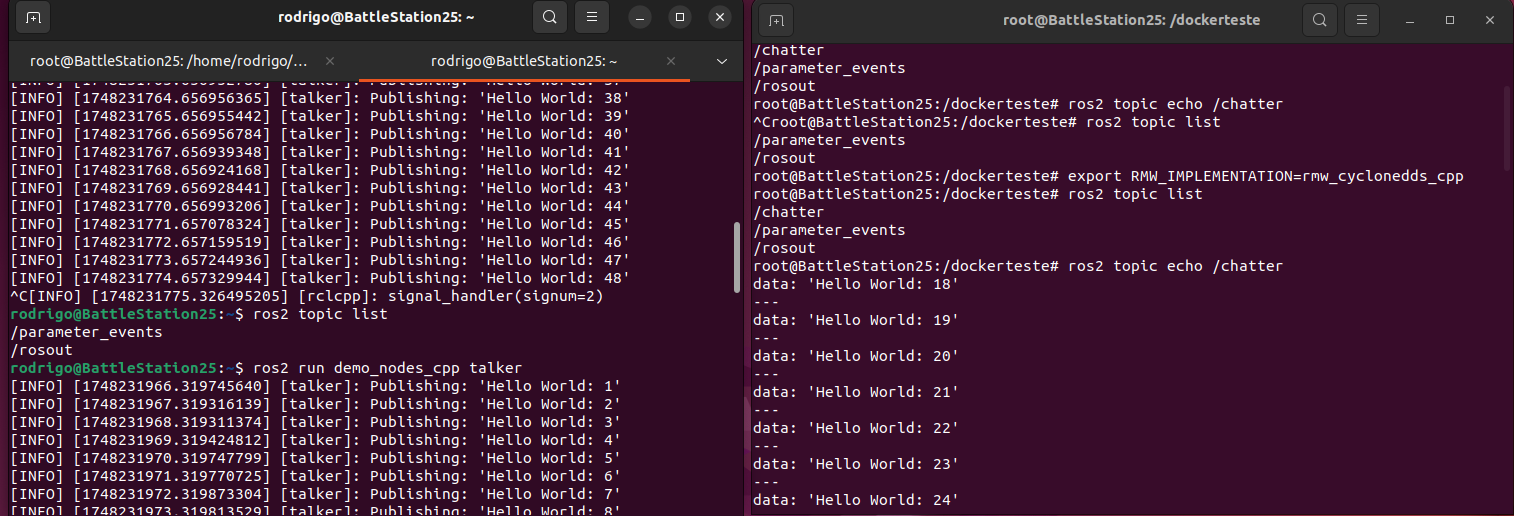
\includegraphics[width=1\linewidth]{Figures/TesteCycloneSucesso.png}
    \caption{Sucesso utilizando RMW CycloneDDS }
    \label{fig:enter-label}
\end{figure}
\begin{figure}[htb]
    \centering
    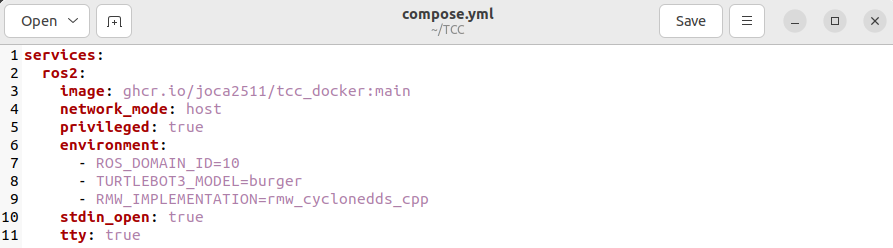
\includegraphics[width=1\linewidth]{Figures/ComposeFinal.png}
    \caption{Compose proposto para testes}
    \label{fig:enter-label}
\end{figure}
\begin{figure}[htb]
    \centering
    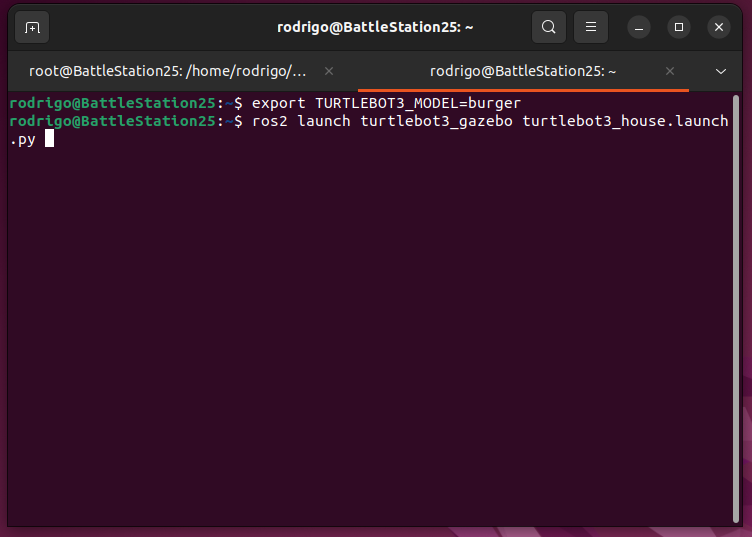
\includegraphics[width=1\linewidth]{Figures/SimulacaoGazeboLancada.png}
    \caption{Simulação Gazebo é lançada pelo host}
    \label{fig:enter-label}
\end{figure}
\begin{figure}[htb]
    \centering
    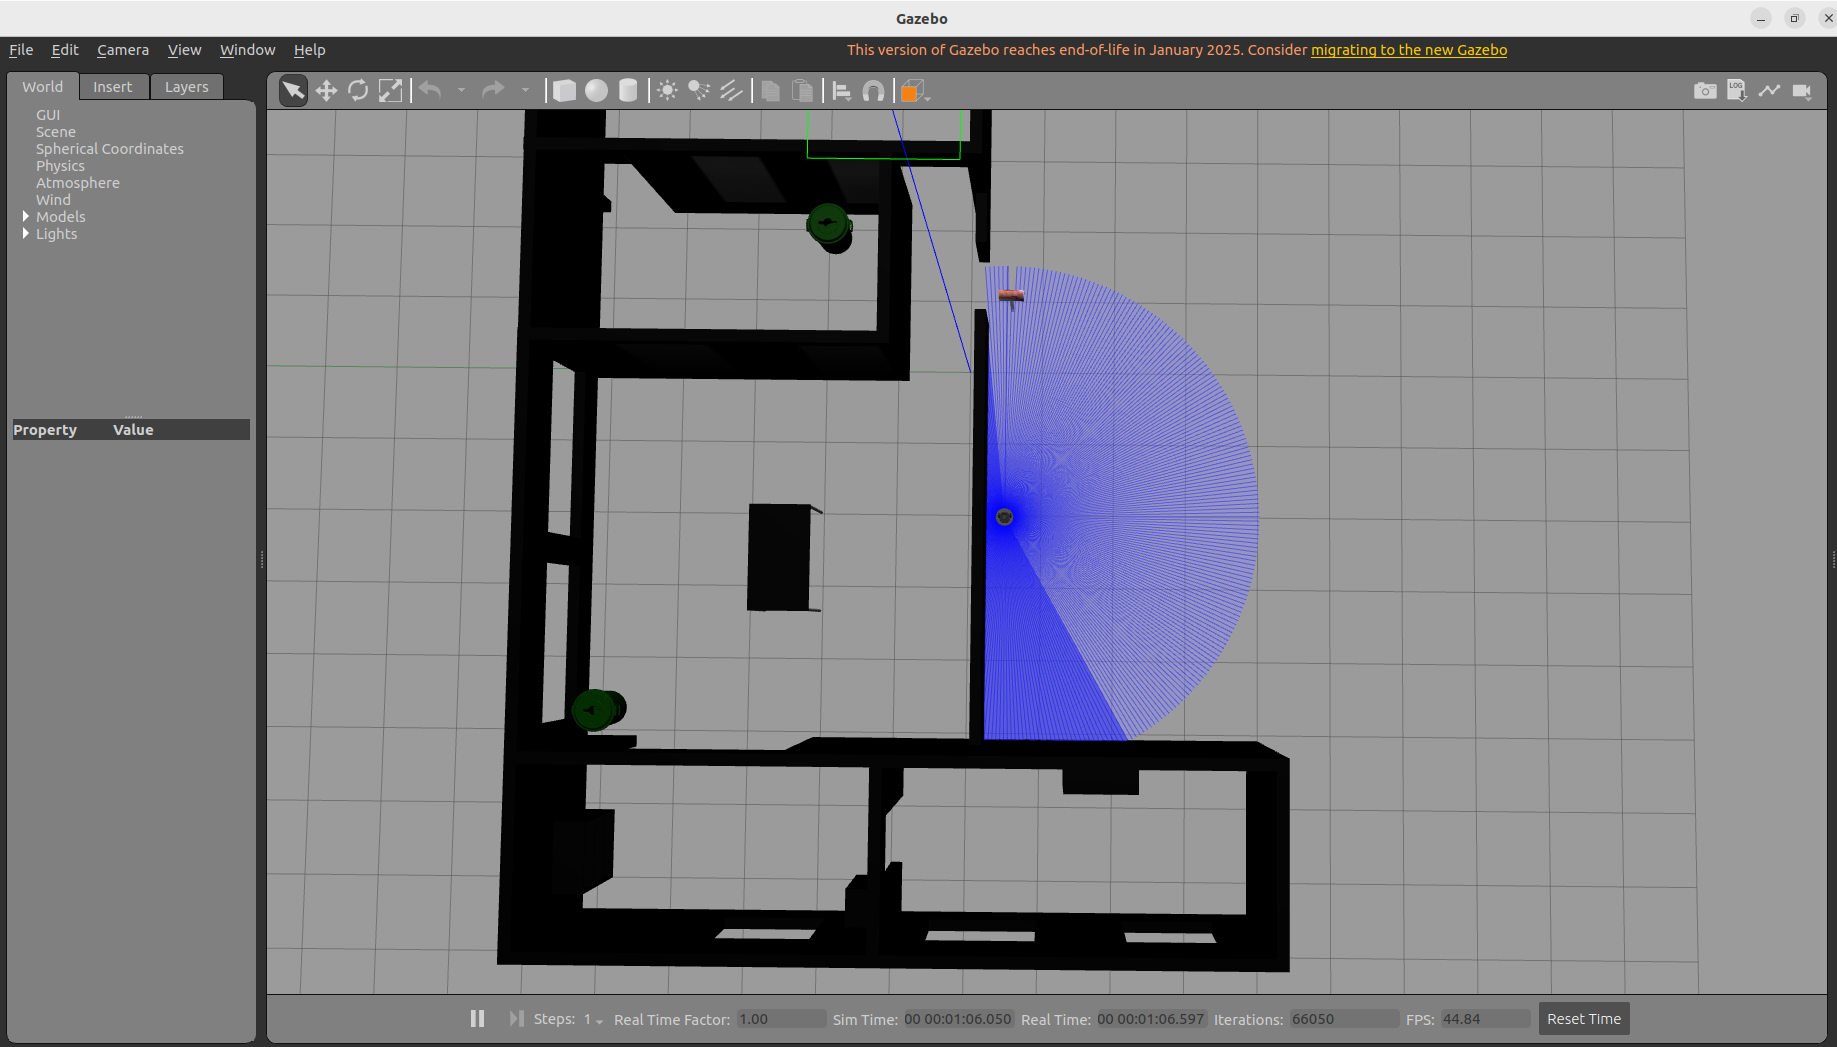
\includegraphics[width=1\linewidth]{Figures/GazeboLancado.png}
    \caption{Aparência inicial da simulação Gazebo}
    \label{fig:enter-label}
\end{figure}
\begin{figure}[htb]
    \centering
    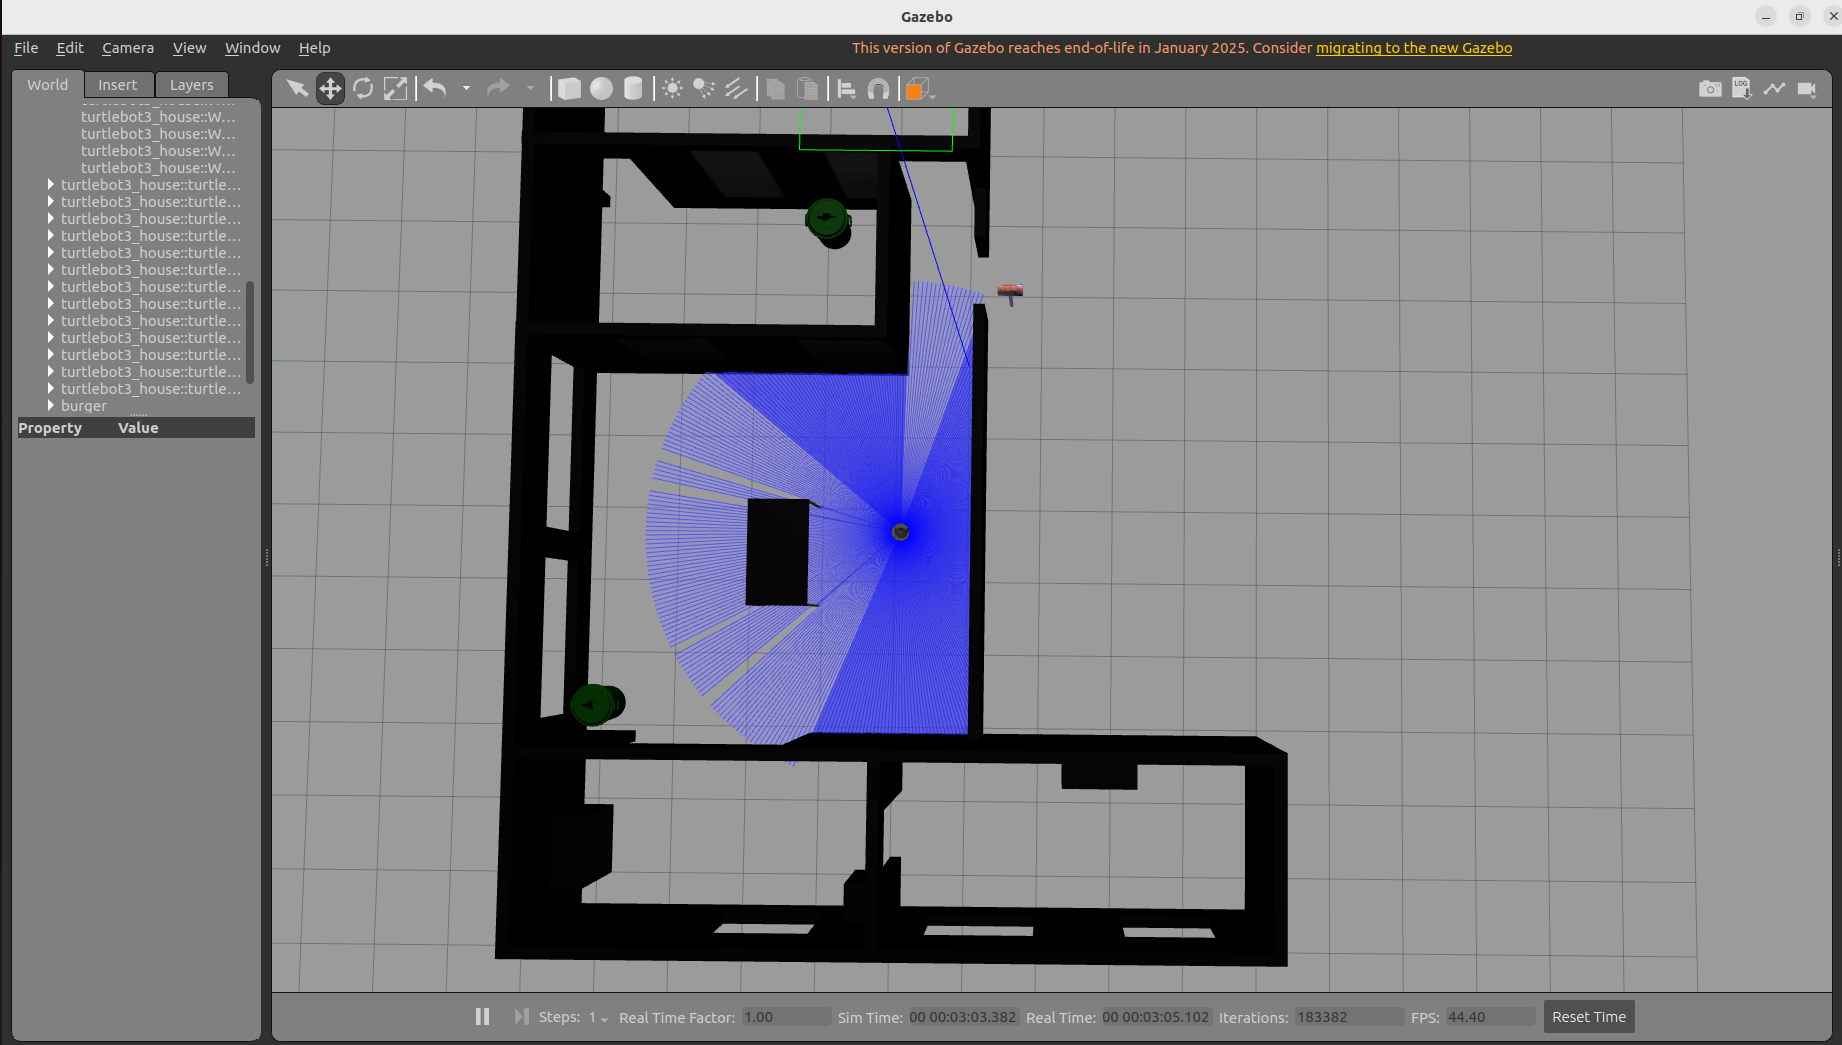
\includegraphics[width=1\linewidth]{Figures/BurgerMovido.png}
    \caption{Turtlebot3 Burger é movido para dentro da casa}
    \label{fig:enter-label}
\end{figure}
\begin{figure}[htb]
    \centering
    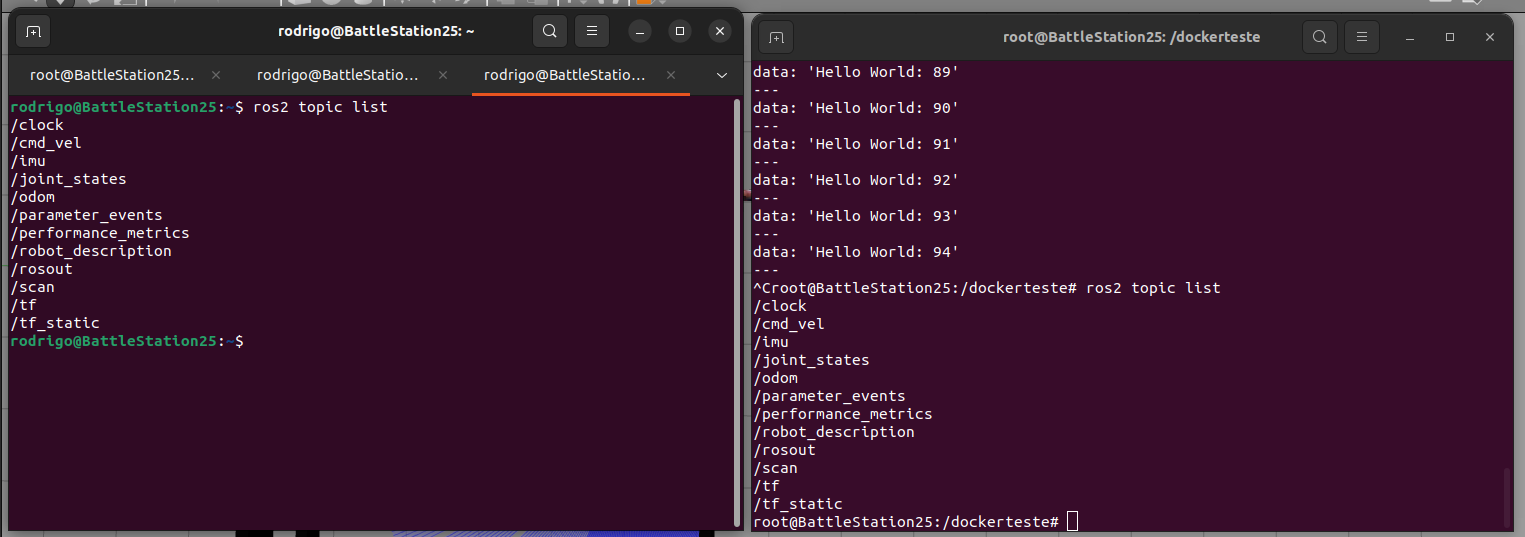
\includegraphics[width=1\linewidth]{Figures/DockerAdquireTopicos.png}
    \caption{ROS2 Humble dentro do Docker adquire os novos tópicos}
    \label{fig:enter-label}
\end{figure}
\begin{figure}[htb]
    \centering
    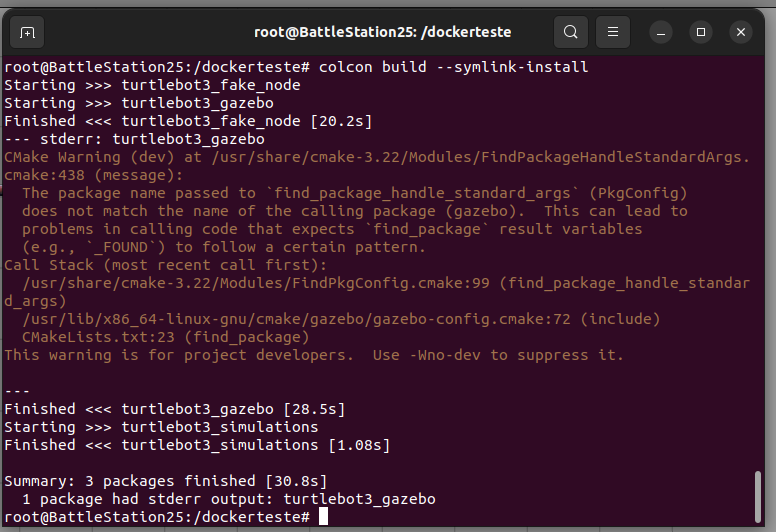
\includegraphics[width=1\linewidth]{Figures/DockerBuildaProjetos.png}
    \caption{ROS2 Humble dentro do Docker builda projetos}
    \label{fig:enter-label}
\end{figure}
\begin{figure}[htb]
    \centering
    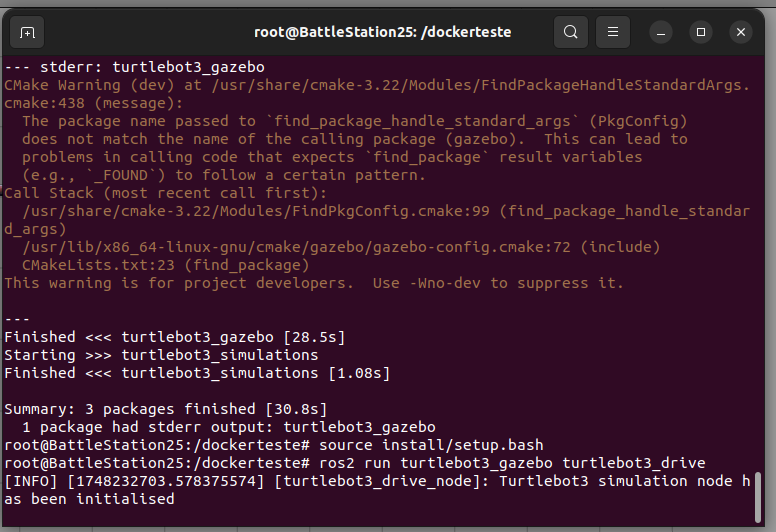
\includegraphics[width=1\linewidth]{Figures/DockerRodaProjetoDrive.png}
    \caption{ROS2 Humble dentro do Docker roda projetos para movimentação do robô dentro da simulação Gazebo presente no host}
    \label{fig:enter-label}
\end{figure}
\begin{figure}[htb]
    \centering
    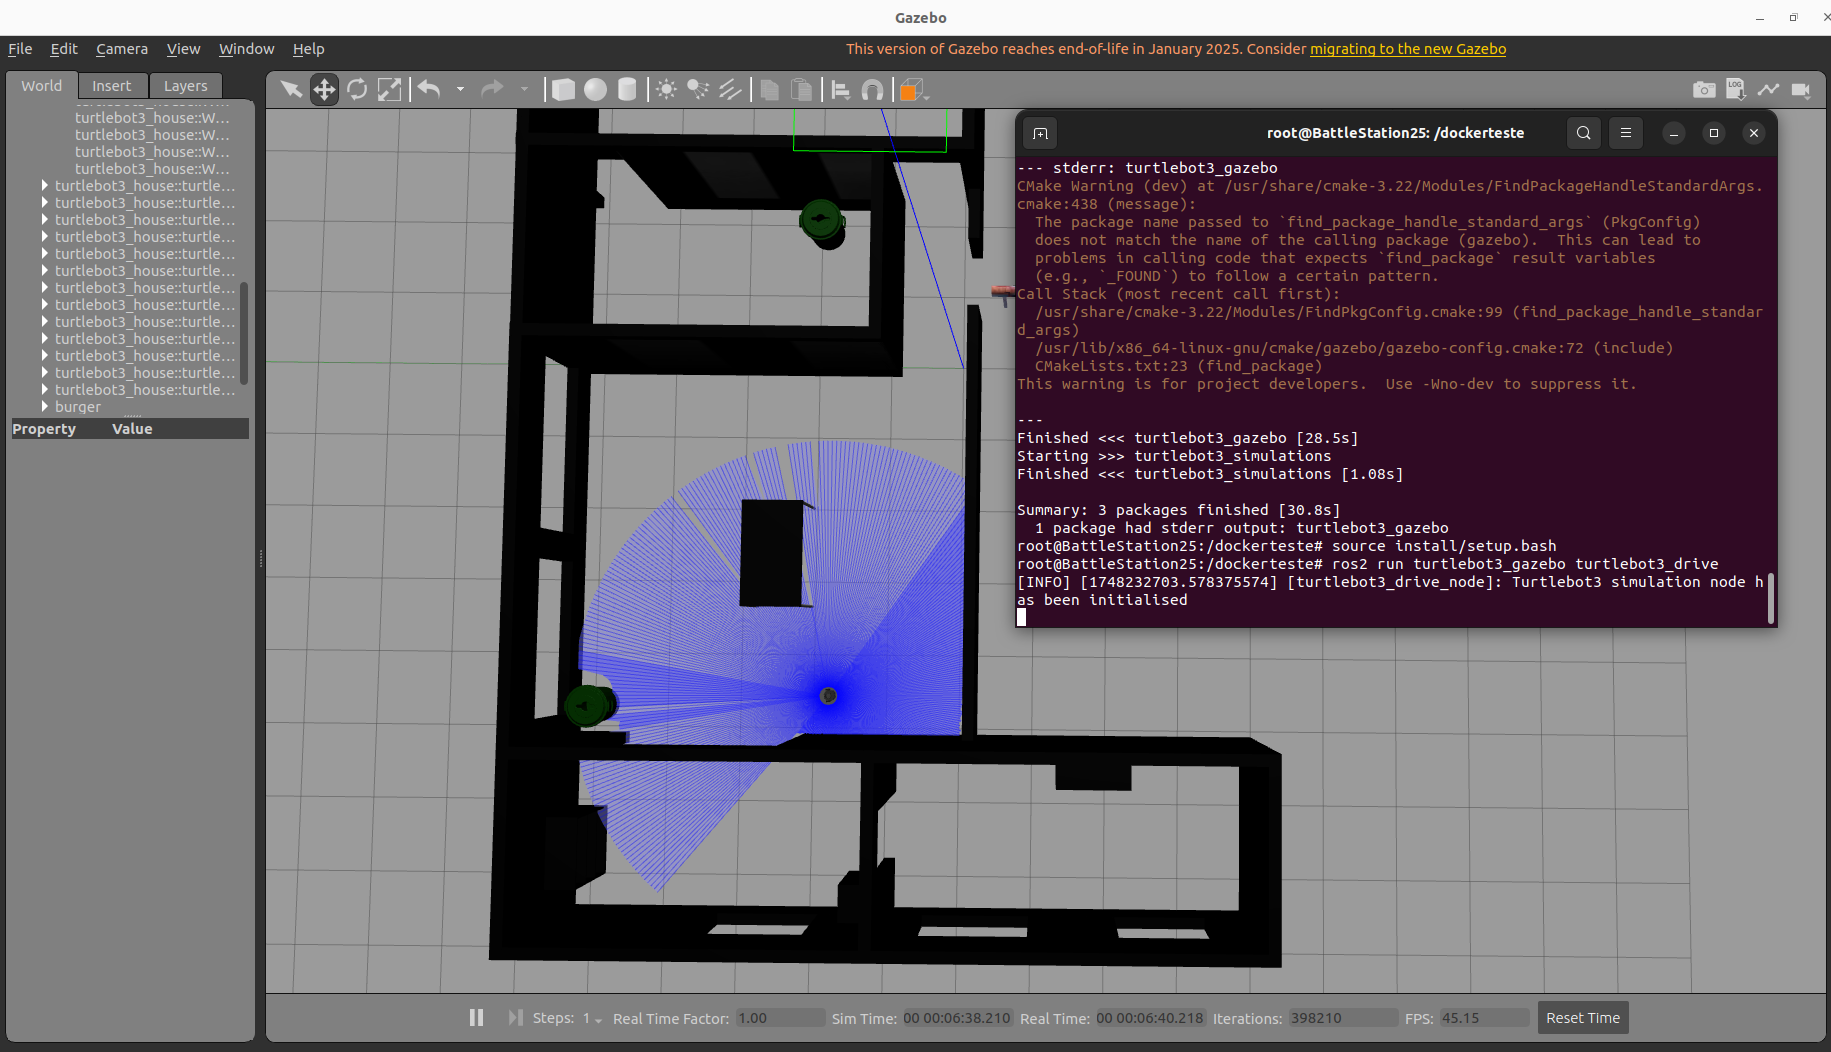
\includegraphics[width=1\linewidth]{Figures/DockerMovimentaRobo1.png}
    \caption{Turtlebot3 Burger é movimentado pelo ROS2 Humble presente dentro do conteiner Docker}
    \label{fig:enter-label}
\end{figure}
\begin{figure}[htb]
    \centering
    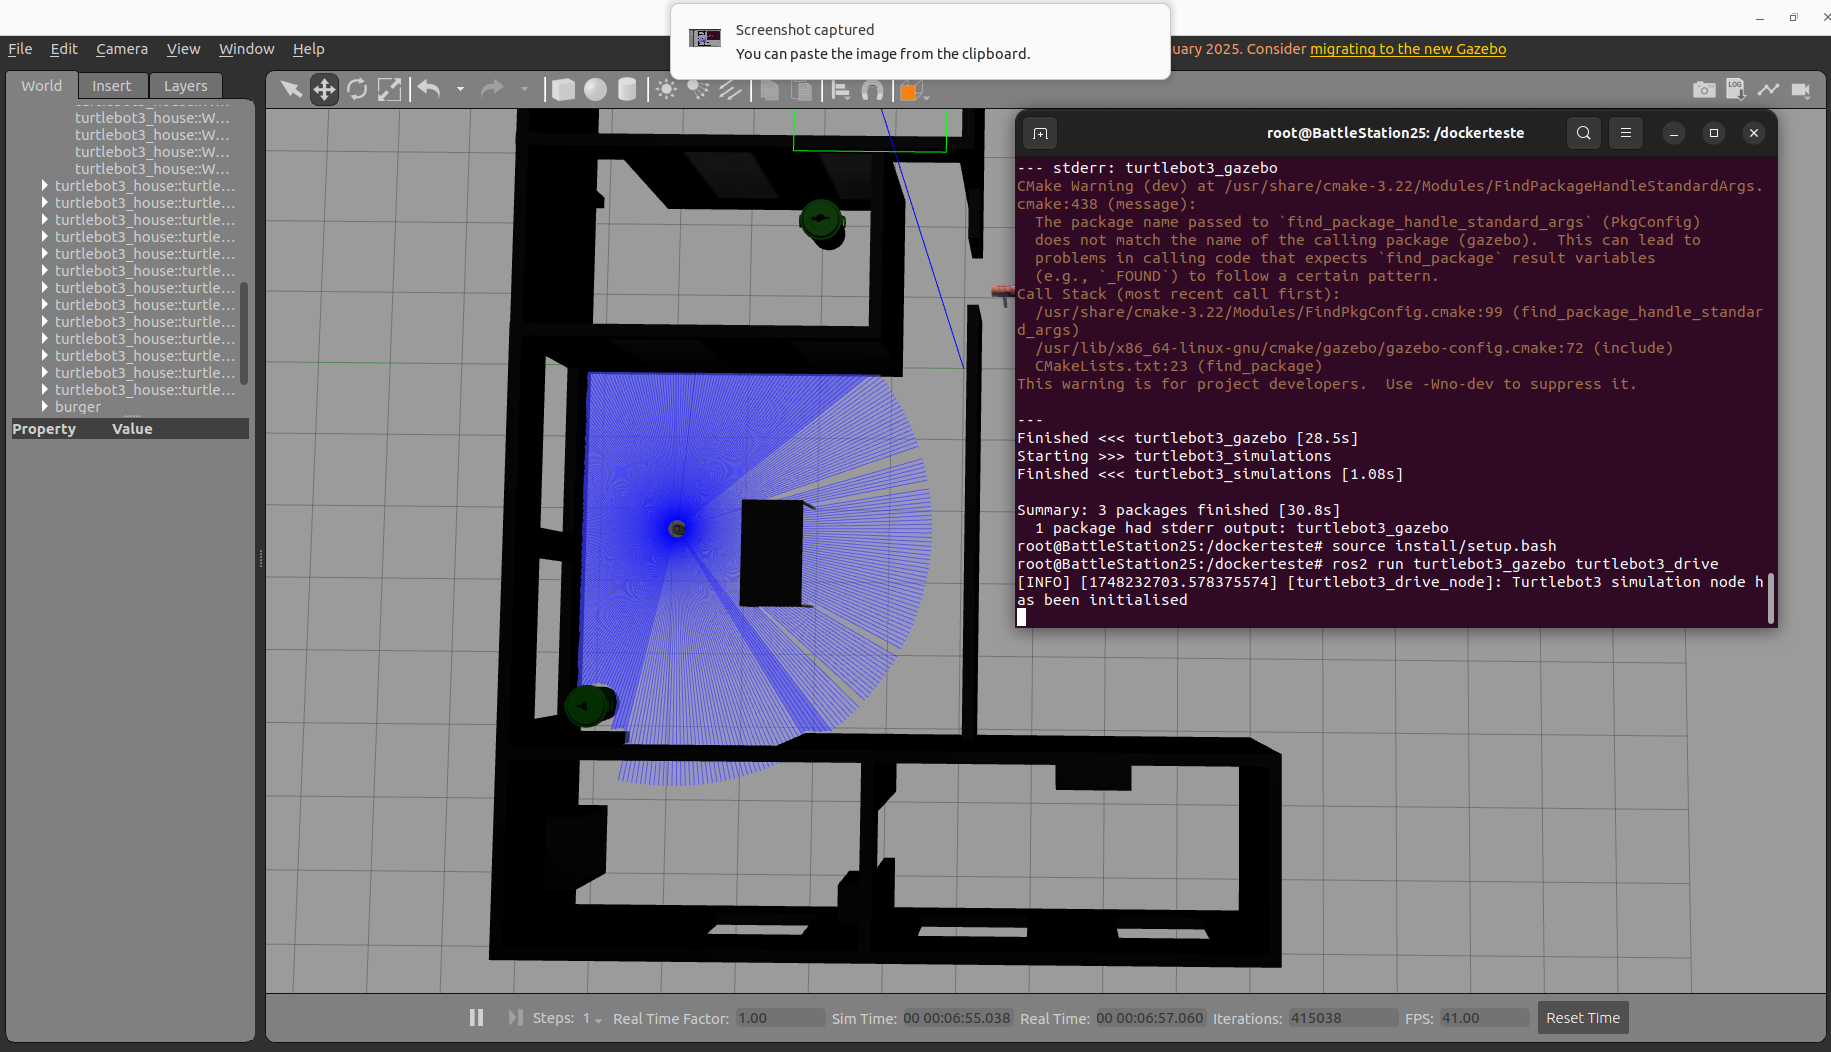
\includegraphics[width=1\linewidth]{Figures/DockerMovimentaRobo2.png}
    \caption{Turtlebot3 Burger é movimentado pelo ROS2 Humble presente dentro do conteiner Docker}
    \label{fig:enter-label}
\end{figure}



% este arquivo aqui pode ser descomentado apenas em TCC2
%\include{tcc-discussao-conslusao}

%\bibliographystyle{plain}
\bibliography{tcc-referencias}
%\addbibresource{tcc-nome-referencias.bib}
%\printbibliography

%\bibliographystyle{apalike}
%\bibliography{tcc-nome-referencias}


%\addbibresource{tcc-nome-referencias}

%\printbibliography

%\printindex

\end{document}